\chapter{Localization under Android}
\label{chap:and-loc}

\section*{Introduction}
The localization of the user is a key function under Android.
It allows for example to directly show the part of the map where the user is on Google Maps, to display advertisements for nearby shops, to automatically select the relevant area for the weather forecast, to gives statistical information of the country usage of an application...
Many applications use it and it is often an asked permission at the installation.\\

The details on the location methods used by the Android system are often unclear.
This chapter will explain how the Android system manage the location of a device and how this has been subject to privacy concerns.
The efficiency and limits of the DroidWatcher application presented in the chapter \ref{chap:droidwatcher} are dependent of the location techniques detailed in this chapter.
As also been verified through experiences several facts concerning the location data storage.

\section{Available techniques}
Depending of the state of the phone, several techniques can be used to locate an Android device.

\subsection{GPS}
\label{sec:loc-gps}

The GPS, for Global Positioning System is a technology based on satellites trilateration\cite{pocketgpsworld}.
GPS satellites are navigating around the earth in a way to maximize the number of visible satellites anywhere at any time.
There is currently 31 working satellites in orbit.
The location-aware device is equipped with a GPS receiver chip.
This receiver will retrieve broadcasted messages from the reachable satellites.
The messages contains :

\begin{itemize}
\item the time the message was transmitted
\item precise orbital information (the ephemeris)
\item the general system health and rough orbits of all GPS satellites (the almanac)
\end{itemize}

Trilateration is used based on the received messages as shown in figure \ref{fig:gps-earth}.
If theoretically, three satellites are enough, at least four is required to avoid clock desynchronization errors (at the speed of light, even an small clock error can lead to huge error).\\

\begin{figure}[h]
  \centering
  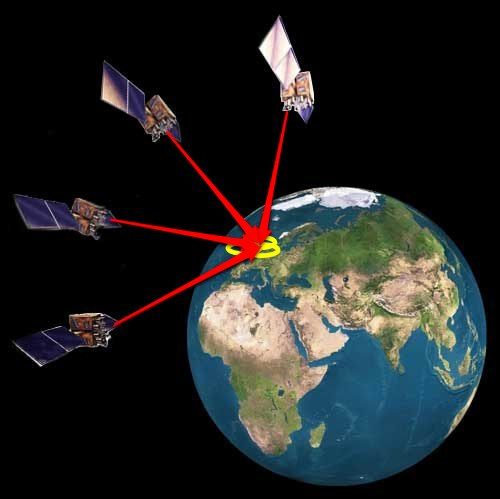
\includegraphics[width=6cm]{images/gps.jpg}
  \caption{Signals from multiple satellites are required to calculate a position\newline Copyright PocketGPSWorld.com}
  \label{fig:gps-earth}
\end{figure}


The accuracy of this method depends of the surrounding of the user.
In clear sight, the accuracy will be of a few meters but it will degrade if the receiver is surrounded by high buildings or inside a dense forest.\\

The time to first fix (TTFF) depends on the state of the GPS.
In a cold start scenario\footnote{Device is in factory state or the GPS data are not relevant (several months old or inaccurate)}, the GPS needs to retrieve the full almanac.
This is done in at least 12.5 minutes\cite{gpsuser}.
To improve the TTFF, embedded GPS often use assisted-GPS technology (aGPS) by acquiring almanac and ephemeris data over a fast network connection when available.

\subsection{Wireless access point}
Each wireless access point has a unique identifier\footnote{BSSID for Basic Service Set IDentification, a unique 48 bit address}.
If the wireless is turned on, the device can retrieve the surrounding access points.
Assuming the geographical coordinates of all the access points are known, it is possible to have an estimation of the location of the user by trilateration.\\

The advantage of this method is that for an accuracy of about 100 meters, the localization is faster than using GPS, consumes less battery power than a GPS receiver chip and does not have other geographical requirements than being surrounded by at least one access point.\\

The collect method used by Google is explained below.

\subsection{Cell tower}
Similar as for the method used with wireless access points, a cell tower as a unique identifier.
On the GSM network, a cell tower is characterized by a Location Area Code and a Cell-ID.
A cellphone can them be located using trilateration based on the surrounding cell towers.\\

In the DroidWatcher application (see chapter \ref{chap:droidwatcher}), the application implements its own trilateration algorithm for offline computation.


\section{Access points and cells databases}
\label{sec:andro-cell-db}

To locate a device using the network resources (using wifi and cell towers, as opposed to the GPS resource), the system needs to access to a database mapping the geographical coordinates of the requested access points and GSM cell tower.
SkyHook, Apple and Google are three companies well know for using such databases.\\

SkyHook was one of the first to create a database to locate wireless access points and developed an SDK to query the location of a user .
The information is collected by war-driving\footnote{Car equipped with a GPS, wireless and cell tower receiver collecting data in the streets} in North America, Western Europe and some Asian countries\cite{skyhook-coverage}.\\

Companies have quickly understood the value of this information and the economical interest of having its own database as a betterment for location aware applications.
While Apple was, at first, using SkyHook, it has now developed its own database system.
Google is also independent and has created its own database.\\

As they collect data to improve the accuracy of their location services, these companies have been subject to criticism recently.
Users wondered about the usage of this database and how it could hurt the privacy of users\footnote{In may 2011 a database containing the location of the last visited access points and cell tower has been discovered inside iPhones. Similar database is also present in Android phones.}.

\subsection{Collect method}
In the case of Google, the location server is constructed based on two factors:
\begin{itemize}
\item Google Cars
\item Crowd-sourcing
\end{itemize}

The Google Cars are mainly used to take pictures to illustrate the service Google Street View.
In addition to that, the cars are also war-driving.
Having a GPS module on the car and driving almost all over the world, it was a good opportunity to constitute a very accurate database.\\

As most Android devices are equipped with a GPS receiver, collecting via crowd-sourcing is also possible.
When an Android device uses the Google database to request a location, data are also transmitted to Google servers.
This way, the database of wireless access points and cell tower is always up to date\footnote{Francisco Kattan, feb 2010, \url{http://franciscokattan.com/2010/02/06/dynamic-cell-id-clever-way-to-block-google-but-will-it-backfire/}}.

\subsection{Location cache files}

Previous cells and access points locations are stored in an unencrypted system files.
This allows to locate the user quickly and still be able to use the network resource, even when the user is not connected to the Internet.
%This local cache file is stored in the folder \texttt{/data/data/com.google.android.location/files} in the files \texttt{cache.wifi} and \texttt{cache.cell}.
Each entries in the cache file is linked with a timestamp representing the date of the retrieval as seen in figure \ref{fig:locmap}.\\

\begin{figure}[h]
  \centering
  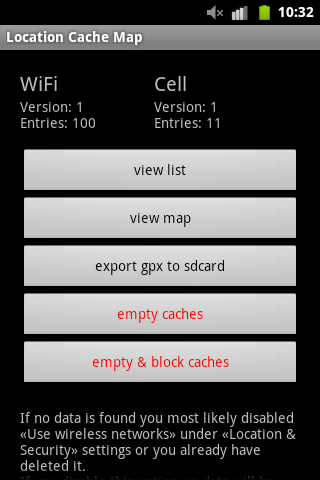
\includegraphics[width=5cm]{images/cache1.png}
  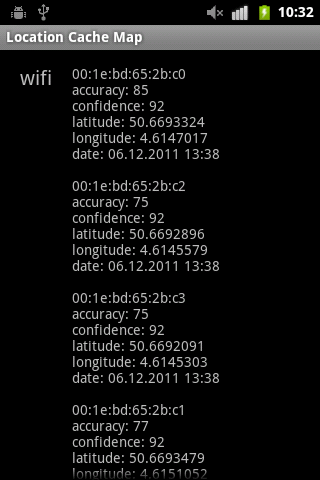
\includegraphics[width=5cm]{images/cache2.png}
  \caption{Captures from the application Location Cache by Remy Demy}
  \label{fig:locmap}
\end{figure}

The recent criticisms about privacy concerns were mainly based on the existence of these cache files.
If the iOS devices used to have unlimited cache size (fixed in iOS 4.3.3), on an Android device, only the 50 last cells and 200 access points have been observed as stored in the cache files.
However, observations made on several devices have shown that this size is enough to contain locations older than one month.
A forensic analysis would allow to retrieve the device location at a given time if a location request was made.
Such requests can be run in background by any application having the correct permission.
The DroidWatcher application relay on this fact to monitor the location of the user in background.\\

To show the ease of retrieving such information, a python script as been developed\cite{soft-locdump} to parse the content of these two files and output a GPS trace file in GPX format representing the approximate movement of the device.
A root access to the phone is however required to access these files\footnote{Most of the time, granting a root access requires a system manipulation and voids the warranty.}.
This could prevent malicious applications to retrieve these data.
Also this cache folder is only composed when the \emph{Use wireless networks} option is enabled in the Android settings, however this option is often required by common applications such as Google Maps which may lead to a large percentage of devices having this option enabled.\\

\subsection{Personal researches}
Several facts about the storage of information and privacy have been announced.
To verify these facts, a set of personal researches have been made.
The applications used to realize the analyses are present in the appendix.

\subsubsection{Database suppression}
When the option \emph{Use wireless networks} is disabled, Google ensured the cache files are deleted.
To ensure the information is deleted from the system when the option is opt out, the following experiment was done:

\begin{enumerate}
\item Make a dump of the internal memory
\item Disable the \emph{Use wireless networks} option
\item Make a dump of the internal memory
\item Compare the two dumps
\end{enumerate}

The goal of the comparison was to ensure that only the folder containing the databases is altered and the information is not stored somewhere else.
The analysis reveal that, with the exception of some irrelevant system files (battery state...) modified, the database files and also Google Maps cache have been deleted.\\

\subsubsection{Analysis of location requests}

When a location is requested on an Android device, the system sends an encrypted request to the Google's location servers.
The Google's servers reply to the request with the location of surrounding GSM cell towers and access points.\\

To understand the content of the requests, two analyses have been made.
The first one aimed to ensure the location informations are stored only in the two cache folders.
The second one is an analysis of the volume of transmitted data correlated to the number of entries added in cache.\\

To ensure that the location information is only stored inside the cache files, the following experiment was done :
\begin{enumerate}
\item Make a dump of the internal memory
\item Request a location update
\item Make a dump of the internal memory
\item Compare the two dumps
\end{enumerate}

The analysis reveal that, with the exception of irrelevant system files, only the database cache files have been modified.\\

The second experiment used the tool tcpdump to correlate a request with the content of the cache files.
The application \emph{LocateMe} has been developed to make a simple location request using the network resources.

\begin{enumerate}
\item Start in \emph{blank state}\footnote{\emph{Blank state} : wireless turned off, empty location cache, location permission turned off, no process requiring the location such as Google Maps running.}
\item Start tcpdump
\item Activate the wireless
\item Request a location with the application \emph{LocateMe}
\item Stop tcpdump once a location received
\end{enumerate}

\begin{figure}[h]
  \hspace*{-2cm}
  \centering
  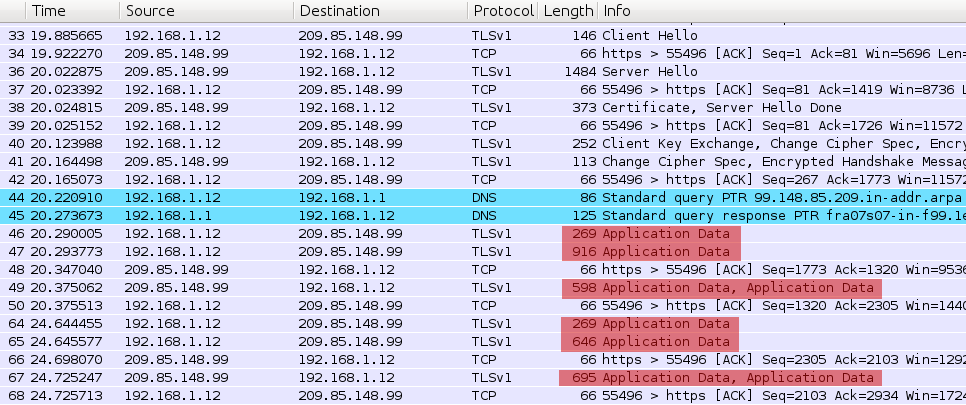
\includegraphics[width=17cm]{images/trace2.png}
  \caption{Example of tcpdump capture while a location request}
  \label{fig:loc-req-tcpdump}
\end{figure}

From the collected trace, the size of the transmitted data was compared with the number of cells and access points added to the cache files.
After observation and repeating the experiment, the following pattern was derived :

\begin{itemize}
\item Two requests are made, one for the cells, one for the wifi.
\item The first packets contains every time 269 bytes.
\item The uploaded data size is larger than the downloaded.
\item The size of the downloaded data is directly linked to the number of entries in the cache files.
\end{itemize}

The figure \ref{fig:loc-req-tcpdump} shows an example of collected trace confirming the derived pattern.
These observations do not allow to validate the suppositions concerning the packet contents but the patterns are coherent to the model explained before.


\section{Privacy concerns}
\subsection{Google Cars}
In May 2010, Google admitted to German authorities having collected more than what it was supposed to.
In addition to access point unique identifier, it had ``been mistakenly collecting samples of payload data from open networks''.
These data chunks could include parts of web surf, email, text...\footnote{TechEYE, may 2012, \url{http://news.techeye.net/security/google-admits-it-sniffed-out-peoples-data}}.
In reaction, the data collected was asked to be deleted and the CNIL (independent French administrative authority) fined Google with €100.000\footnote{BBC UK, mar 2011, http://www.bbc.co.uk/news/technology-12809076}.\\

\subsection{\_nomap}

Some users considered the automatically collected data by the Google Cars and Android devices as private.
In November 2011, in reaction to criticism, Google created a way to opt out recording of its access point.
The proposition of Google is to end the ESSID of the wireless access point with \texttt{\_nomap}.
The next time it will be scanned by a Google Cars or an Android device, the access point will be removed from the database.
Google hopes than over time, the \texttt{\_nomap} string will be adopted by other location providers\cite{nomap}.\\

This proposition was received with much scepticism and did not satisfied the pro-privacy groups.
The main complain was the need of an action from the user to explicitly opt out its access point while people wanted a way to explicitly opt in instead.
Many people that are concerned by privacy issues do not have enough technical knowledge to modify the wireless network name.
Furthermore, if this string is not universally adopted by other companies such as Apple or SkyHook, conflicting systems can be imagined, preventing a concerned user to fully opt out its access points from commercial databases.

\subsection{Research of Samy Kamkar}

To reply to privacy concerns, Google ensured ``The location information sent to Google servers when users opt in to location services on Android is anonymized and stored in the aggregate and is not tied or traceable to a specific user''\cite{loc-not-traceable}.
The security researcher Samy Kamkar has also looked at the location requested.\\

\begin{figure}[h]
  \hspace*{-2cm}
  \centering
  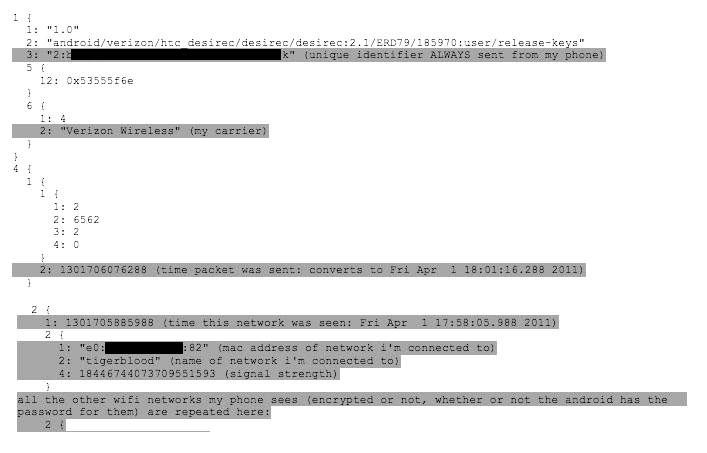
\includegraphics[width=18cm]{images/reqdecode.jpg}
  \caption{Decrypted request content reveal to CNet by Samy Kamkar}
  \label{fig:reqdecode}
\end{figure}

He succeeded to decrypt the request made to Google servers and realized that it contains a unique identifier\cite{cnet-andr-samy}.
The figure \ref{fig:reqdecode} is the content of a request decrypted by Samy Kamkar sent to CNet.
The identifier is unique to the cell phone and present in every request.
If this string does not directly reveal the identity of the phone owner, it is however possible to tied the string to a specific user and then trace him.
He affirms there is no proof the location is anonymized due to the presence of this identifier.\\

Personal researches showed that this string is contained inside a file next to the cache database and it is renewed every time the \emph{Use wireless networks} option is toggled.
%\texttt{/data/data/com.google.android.location/files/gls.platform.key} 
If it is relatively easy to change this value, we can imagine that very few users are aware of the existence of this value and will apply this manipulation regulary.
% \subsection{Android API}
% When an application wants to locate the device position, the Android system provides some higher level methods to use the available technologies listed above. Getting a user location in Android works by means of callback. A \texttt{LocationListener} is defined and will react to event such as \texttt{onLocationChanged} or \texttt{onProviderEnabled}. On the relevent event, the callback function is executed and the location retrieved \cite{doc-location}.

% \lstset{language=Java}
% \begin{lstlisting}[label=location-base,caption=Code from Android developers guide]
% // Acquire a reference to the system Location Manager
% LocationManager locationManager = (LocationManager) this.getSystemService(Context.LOCATION_SERVICE);

% // Define a listener that responds to location updates
% LocationListener locationListener = new LocationListener() {
%     public void onLocationChanged(Location location) {
%       // Called when a new location is found by the network location provider.
%       makeUseOfNewLocation(location);
%     }

%     public void onStatusChanged(String provider, int status, Bundle extras) {}

%     public void onProviderEnabled(String provider) {}

%     public void onProviderDisabled(String provider) {}
%   };

% // Register the listener with the Location Manager to receive location updates
% locationManager.requestLocationUpdates(LocationManager.NETWORK_PROVIDER, 0, 0, locationListener);
% \end{lstlisting}
  
% At any moment, a user can request the last known location using the following code

% \begin{lstlisting}[label=getLastKnown,caption=Get the last recorded location]
% LocationProvider locationProvider = LocationManager.NETWORK_PROVIDER;
% // Or use LocationManager.GPS_PROVIDER

% Location lastKnownLocation = locationManager.getLastKnownLocation(locationProvider);
% \end{lstlisting}

% The provider \texttt{GPS\_PROVIDER}  or \texttt{NETWORK\_PROVIDER} allows to choose the source of the location. The GPS is used in the first case and an hybrid method using both wireless and cell tower location in the second.\\

% A \texttt{Location} is characterized by the following parameter that can be used to determined if a location is or not relevant by an application :
% \begin{itemize}
% \item Logitude
% \item Latitude
% \item Altitude
% \item Provider (GPS, Network...)
% \item Accuracy
% \item Time of the fix
% \end{itemize}
